\chapterpage\chapter{Evaluation}
        In diesem Abschnitt wird anhand der SMAPE-Metrik quantifiziert, wie viel die Leistung des Modells verbessert, indem die Ausreißer durch die vorgeschlagene Methode entfernt werden, und das Ergebnisse werden diskutiert.
        
        Bevor die Leistungsänderungen des Modells für jede Methode aufgeführt werden, wird die Metrik SMAPE, die im Schritt „Evaluierung“ des Abschnitts \ref{sec:Modellierung der Feinstaubkonzentration} erwähnt wird und die ein Kriterium für die Evaluierung darstellt, ausführlich erläutert.
        
        \section*{SMAPE}
        
        \section*{Ergebnisse}

            

            


            \begin{figure}[h]
                \centering
                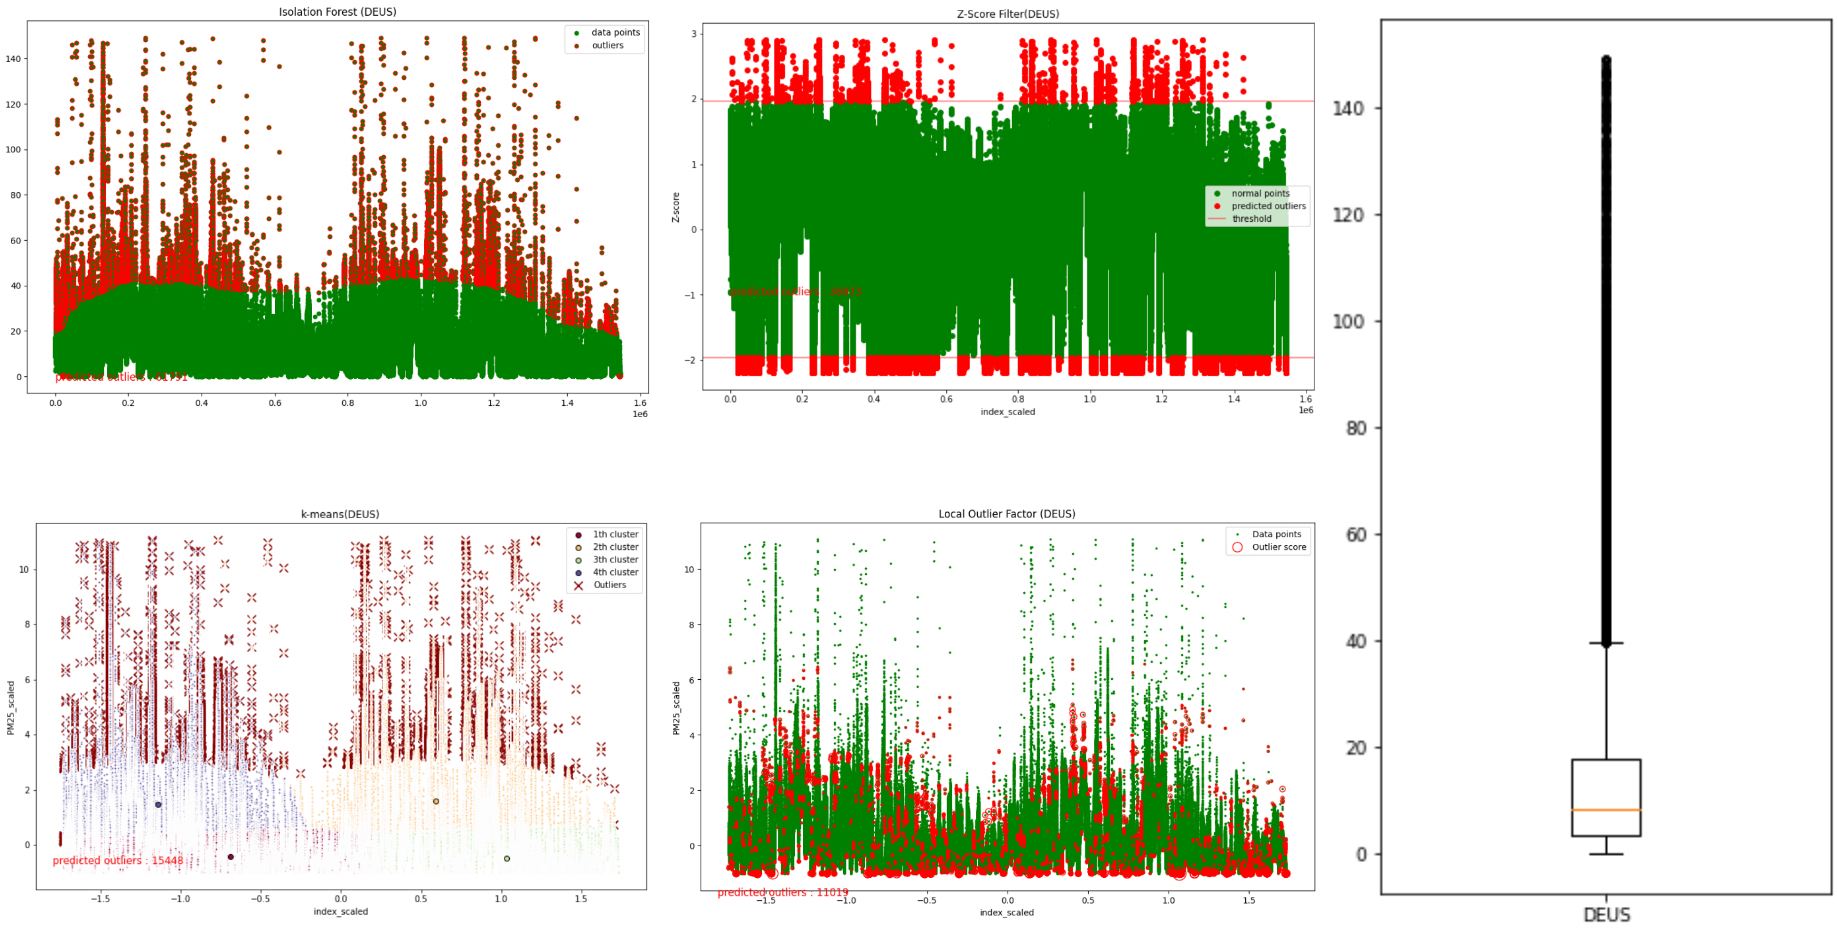
\includegraphics[\linewidth]{images/Visualisierung der Ausreißers.jpg}
                \caption{Visualisierung der Ausreißers}
                \label{fig:Visualisierung der Ausreißers}
            \end{figure}